% Experimental setup and comparison logic only; findings are deferred.
% Provenance and scope: experimental-notes.md.
\section{Experimental study}
\label{sec:experiments}

We examine how pressure's effects on quality and model-wide sparsity depend
on thresholding and placement, and whether an explanation of those effects
transfers across model sizes.
We pretrain randomly initialized Pythia-14M, 70M, and 410M
models~\citep{biderman2023pythia} on MiniPile~\citep{kaddour2023minipile}.
Their shared parallel attention and FFN architecture gives the sites a
consistent interpretation across sizes. Detailed comparisons use 14M;
the larger models cover selected recipes. We pair validation cross-entropy
and $\Smodel$ from the same checkpoint and forward configuration.
Appendix~\ref{app:experiment} specifies the architecture and evaluation details.

% Existing setup artifact; moved here without changing its content.
\begin{figure}[htbp]
\centering
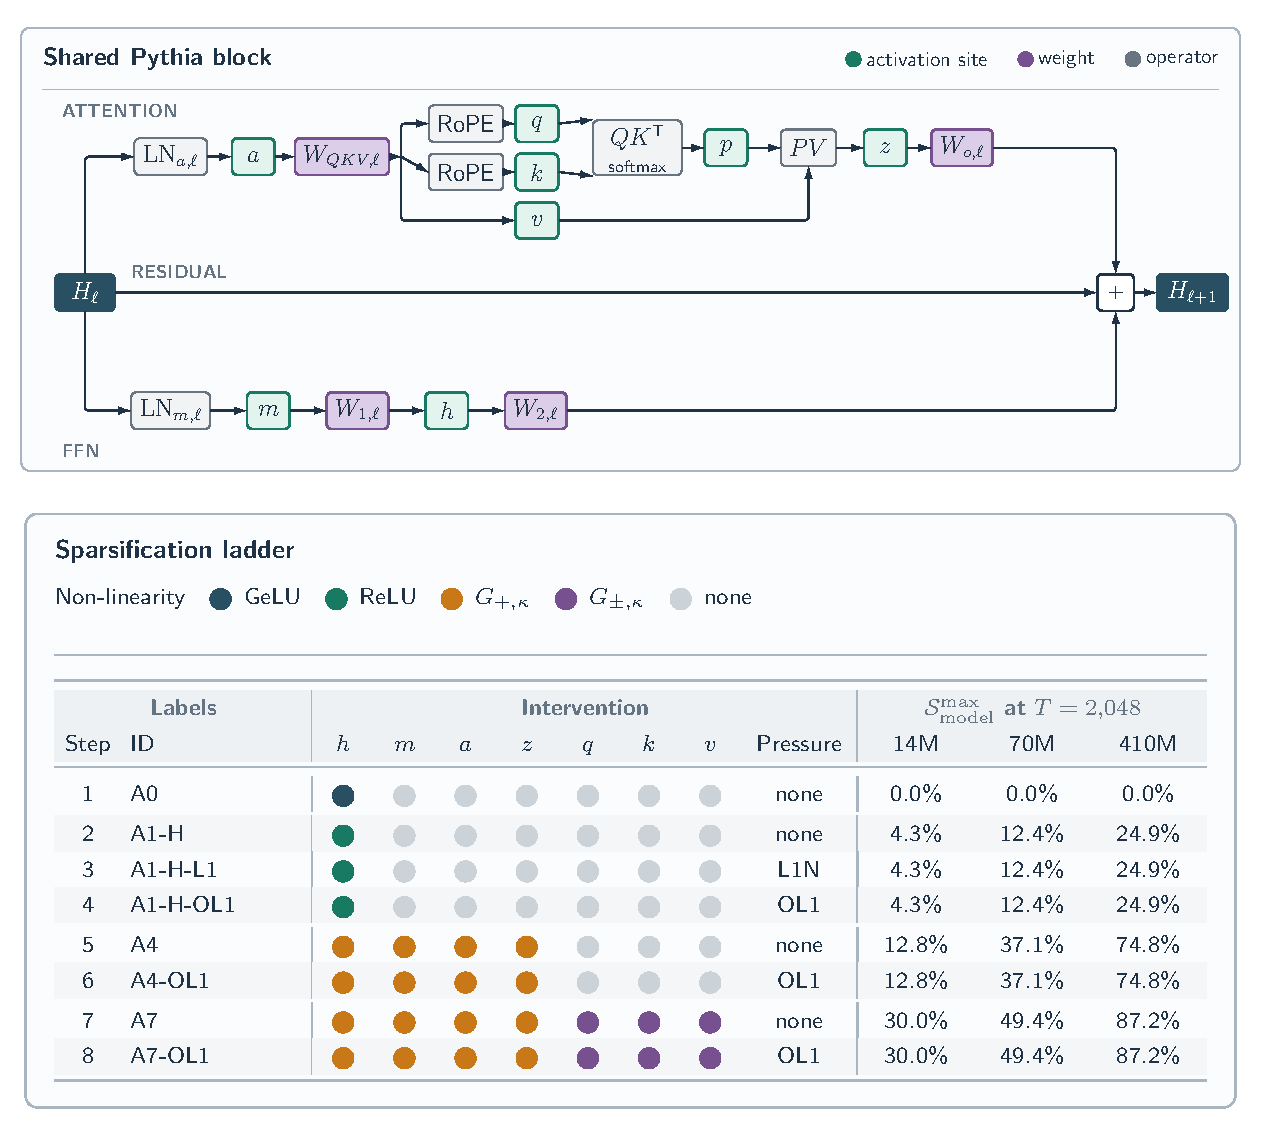
\includegraphics[width=\linewidth]{../artifacts/pythia-architecture-sparsification-ladder.pdf}
\caption{Shared Pythia block and sparsification intervention ladder.
The map separates gate placement, gate family, and pressure; L1N denotes
naive L1. The final columns show analytic selected-site reach $100\Smax\%$
at $T=2{,}048$, not observed sparsity or speedup. Pressure targets all gated
sites in each pressure-bearing row. Rows define candidate recipes; their
experimental coverage is reported with the results.}
\label{fig:intervention-ladder}
\end{figure}


Figure~\ref{fig:intervention-ladder} locates the normalized attention and
FFN inputs ($a,m$), FFN hidden activation ($h$), concatenated attention
context ($z$), and query, key, and value operands ($q,k,v$).
Query and key gates follow rotary position encoding (RoPE); $z$ precedes
the attention-output projection. A0 retains the stock block. A1-H replaces
GELU at $h$ with ReLU; A4 applies one-sided thresholding at $\{a,m,h,z\}$;
A7 adds symmetric gates at $\{q,k,v\}$. The L1/OL1 variants apply pressure
to all gated sites in their row. These are separately pretrained conditions,
not stages of a training curriculum. The ladder includes each recipe's
analytic reach, which changes with model architecture.

Within each size, matched contrasts share initialization, data order, and
training budget. Adding pressure at fixed gates measures its additional
quality and sparsity effects; repeating the contrast across thresholds tests
how those effects depend on thresholding. Comparing A4 with A7 without
pressure examines broader gate placement. A4-OL1 versus A7-OL1 changes both
gate and pressure sets, so it compares complete recipes rather than isolating
gate placement at a fixed pressure objective. At 70M and 410M, we evaluate
A0, A1-H, A4-OL1, and A7-OL1 with the same training-token budget as at 14M. Comparisons use one initialization seed
per size; thresholds are treatment levels, not statistical replicates.
Across sizes, we examine each operation's zero-product fraction and its share
of the model workload to interpret changes in $\Smodel$ alongside $\Smax$.

